\documentclass[tikz]{standalone}

\usepackage{fp}
\usepackage{tikz}
\usepackage{tikz-3dplot}
\usepackage{amsmath} %математические формулы
\usepackage[e]{esvect}  %Красивая стрелочка вектора


\usetikzlibrary{calc}
\usetikzlibrary{arrows.meta}

\begin{document}
	
	\newcommand{\VARPOINT}[4] 
	{
		\coordinate (#1) at (#2,#3,#4);
		\coordinate (#1xy) at (#2,#3,0);
		\coordinate (#1xz) at (#2,0,#4);
		\coordinate (#1yz) at (0,#3,#4);
		\coordinate (#1x) at (#2,0,0);
		\coordinate (#1y) at (0,#3,0);
		\coordinate (#1z) at (0,0,#4);
		
		
		\expandafter\edef\csname #1x\endcsname{#2}
		\expandafter\edef\csname #1y\endcsname{#3}
		\expandafter\edef\csname #1z\endcsname{#4}
		
	}
	
	\newcommand{\VECTOR}[2]
	{
		
		\FPset{\x}{0}
		\FPset{\y}{0}
		\FPset{\z}{0}
		\FPsub{\x}{\csname #2x\endcsname}{\csname #1x\endcsname}
		\FPsub{\y}{\csname #2y\endcsname}{\csname #1y\endcsname}
		\FPsub{\z}{\csname #2z\endcsname}{\csname #1z\endcsname}
		
		
		%\expandafter\VARPOINT {vec#1#2}{\csname #1x}{0}{0}
		\expandafter\VARPOINT {vec#1#2}{\x}{\y}{\z}
	}
	
	\newcommand{\VIPI}[2]
	{
		\def\tmpax{\csname#1x\endcsname}
		\def\tmpay{\csname#1y\endcsname}
		\def\tmpaz{\csname#1z\endcsname}
		
		\def\tmpbx{\csname#2x\endcsname}
		\def\tmpby{\csname#2y\endcsname}
		\def\tmpbz{\csname#2z\endcsname}
		
		\FPeval{\resultx}{\tmpay * \tmpbz - \tmpaz * \tmpby}
		\FPeval{\resulty}{\tmpaz * \tmpbx - \tmpax * \tmpbz}
		\FPeval{\resultz}{\tmpax * \tmpby - \tmpay * \tmpbx}
		
		\expandafter\VARPOINT {vp#1#2}{\resultx}{\resulty}{\resultz}	
		
	}
	
	
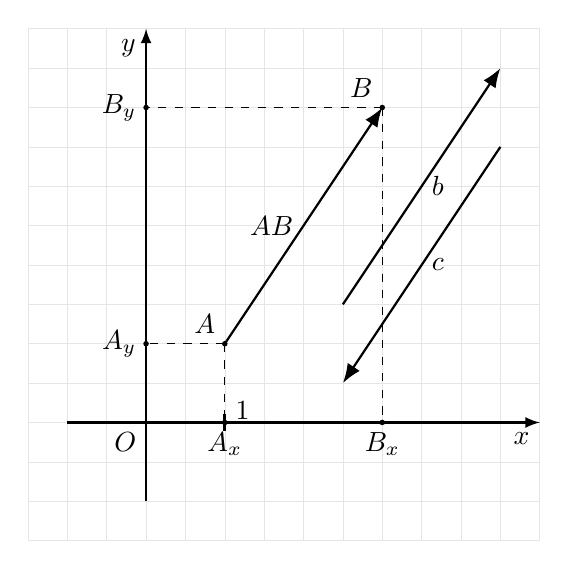
\begin{tikzpicture}[scale=1]
	
	
	\draw[step=.5cm,black!10,very thin] (-1.5,-1.5) grid (5,5);
	
	\draw[-latex, thick] (-1,0) -- (5,0)  node [below left] {$x$};
	\draw[-latex, thick] (0,-1) -- (0,5)  node [below left] {$y$};
	
	\coordinate (O) at (0,0);
	
	\draw (O) node [below left] {$O$};
	
	
	\coordinate (A) at (1,1);
	\coordinate (B) at (3,4);
	\coordinate (Ax) at (A |- O);
	\coordinate (Ay) at (A -| O);
	\coordinate (Bx) at (B |- O);
	\coordinate (By) at (B -| O);
	
	\fill [black] (A) circle [radius=1pt];
	\fill [black] (B) circle [radius=1pt];
	\fill [black] (Ax) circle [radius=1pt];
	\fill [black] (Ay) circle [radius=1pt];
	\fill [black] (Bx) circle [radius=1pt];
	\fill [black] (By) circle [radius=1pt];
	
	\draw[-{Latex[length=7pt]}, thick] (A) -- (B) node [left, midway] {$\vv{AB}$};
	
	\draw (A) node[above left,] {$A$};
	\draw (B) node[above left] {$B$};
	
	\draw (Ax) node [below] {$A_x$};
	\draw (Ay) node [left] {$A_y$};
	\draw (Bx) node [below] {$B_x$};
	\draw (By) node [left] {$B_y$};
	
	
	\draw[dashed] (A) -- (Ax);
	\draw[dashed] (A) -- (Ay);
	\draw[dashed] (B) -- (By);
	\draw[dashed] (B) -- (Bx);
	
	\draw[-{Latex[length=7pt]}, thick] ($(A)+(1.5,0.5)$) -- ($(B)+(1.5,0.5)$) node [right, midway] {$\vv{b}$};
	
	
	\draw[{Latex[length=7pt]}-, thick] ($(A)+(1.5,-0.5)$) -- ($(B)+(1.5,-0.5)$) node [right, midway] {$\vv{c}$};
	
	
	\draw [very thick] (1,0) -- +(up:3pt) -- +(down:3pt) node [above right] {1};
	
	
	
	
	
\end{tikzpicture}
	
\end{document}